\documentclass{beamer}
%\documentclass[xcolor=pst,dvips,epic,eepic]{beamer}

\usepackage[utf8]{inputenc}
\usetheme{Singapore}
\usepackage{xcolor}
\setbeamertemplate{footline}[frame number]

%\usepackage{pgf,pgfarrows,pgfnodes,pgfautomata,pgfheaps,pgfshade}
%\usepackage[pst]{xcolor}
%\usepackage{xxcolor}
% We add the following commonly used macros:

% vectors as boldsymbols:
\newcommand{\bsa}{{\boldsymbol{a}}}
\newcommand{\bsb}{{\boldsymbol{b}}}
\newcommand{\bsc}{{\boldsymbol{c}}}
\newcommand{\bsd}{{\boldsymbol{d}}}
\newcommand{\bse}{{\boldsymbol{e}}}
\newcommand{\bsf}{{\boldsymbol{f}}}
\newcommand{\bsg}{{\boldsymbol{g}}}
\newcommand{\bsh}{{\boldsymbol{h}}}
\newcommand{\bsi}{{\boldsymbol{i}}}
\newcommand{\bsj}{{\boldsymbol{j}}}
\newcommand{\bsk}{{\boldsymbol{k}}}
\newcommand{\bsl}{{\boldsymbol{l}}}
\newcommand{\bsm}{{\boldsymbol{m}}}
\newcommand{\bsn}{{\boldsymbol{n}}}
\newcommand{\bso}{{\boldsymbol{o}}}
\newcommand{\bsp}{{\boldsymbol{p}}}
\newcommand{\bsq}{{\boldsymbol{q}}}
\newcommand{\bsr}{{\boldsymbol{r}}}
\newcommand{\bss}{{\boldsymbol{s}}}
\newcommand{\bst}{{\boldsymbol{t}}}
\newcommand{\bsu}{{\boldsymbol{u}}}
\newcommand{\bsv}{{\boldsymbol{v}}}
\newcommand{\bsw}{{\boldsymbol{w}}}
\newcommand{\bsx}{{\boldsymbol{x}}}
\newcommand{\bsy}{{\boldsymbol{y}}}
\newcommand{\bsz}{{\boldsymbol{z}}}
\newcommand{\bsA}{{\boldsymbol{A}}}
\newcommand{\bsB}{{\boldsymbol{B}}}
\newcommand{\bsC}{{\boldsymbol{C}}}
\newcommand{\bsD}{{\boldsymbol{D}}}
\newcommand{\bsE}{{\boldsymbol{E}}}
\newcommand{\bsF}{{\boldsymbol{F}}}
\newcommand{\bsG}{{\boldsymbol{G}}}
\newcommand{\bsH}{{\boldsymbol{H}}}
\newcommand{\bsI}{{\boldsymbol{I}}}
\newcommand{\bsJ}{{\boldsymbol{J}}}
\newcommand{\bsK}{{\boldsymbol{K}}}
\newcommand{\bsL}{{\boldsymbol{L}}}
\newcommand{\bsM}{{\boldsymbol{M}}}
\newcommand{\bsN}{{\boldsymbol{N}}}
\newcommand{\bsO}{{\boldsymbol{O}}}
\newcommand{\bsP}{{\boldsymbol{P}}}
\newcommand{\bsQ}{{\boldsymbol{Q}}}
\newcommand{\bsR}{{\boldsymbol{R}}}
\newcommand{\bsS}{{\boldsymbol{S}}}
\newcommand{\bsT}{{\boldsymbol{T}}}
\newcommand{\bsU}{{\boldsymbol{U}}}
\newcommand{\bsV}{{\boldsymbol{V}}}
\newcommand{\bsW}{{\boldsymbol{W}}}
\newcommand{\bsX}{{\boldsymbol{X}}}
\newcommand{\bsY}{{\boldsymbol{Y}}}
\newcommand{\bsZ}{{\boldsymbol{Z}}}
% other commonly used boldsymbols:
\newcommand{\bsell}{{\boldsymbol{\ell}}}
\newcommand{\bszero}{{\boldsymbol{0}}} % vector of zeros
\newcommand{\bsone}{{\boldsymbol{1}}}  % vector of ones
% boldsymbol greeks:
\newcommand{\bsalpha}{{\boldsymbol{\alpha}}}
\newcommand{\bsbeta}{{\boldsymbol{\beta}}}
\newcommand{\bsgamma}{{\boldsymbol{\gamma}}}
\newcommand{\bsdelta}{{\boldsymbol{\delta}}}
\newcommand{\bsepsilon}{{\boldsymbol{\epsilon}}}
\newcommand{\bsvarepsilon}{{\boldsymbol{\varepsilon}}}
\newcommand{\bszeta}{{\boldsymbol{\zeta}}}
\newcommand{\bseta}{{\boldsymbol{\eta}}}
\newcommand{\bstheta}{{\boldsymbol{\theta}}}
\newcommand{\bsvartheta}{{\boldsymbol{\vartheta}}}
\newcommand{\bskappa}{{\boldsymbol{\kappa}}}
\newcommand{\bslambda}{{\boldsymbol{\lambda}}}
\newcommand{\bsmu}{{\boldsymbol{\mu}}}
\newcommand{\bsnu}{{\boldsymbol{\nu}}}
\newcommand{\bsxi}{{\boldsymbol{\xi}}}
\newcommand{\bspi}{{\boldsymbol{\pi}}}
\newcommand{\bsvarpi}{{\boldsymbol{\varpi}}}
\newcommand{\bsrho}{{\boldsymbol{\rho}}}
\newcommand{\bsvarrho}{{\boldsymbol{\varrho}}}
\newcommand{\bssigma}{{\boldsymbol{\sigma}}}
\newcommand{\bsvarsigma}{{\boldsymbol{\varsigma}}}
\newcommand{\bstau}{{\boldsymbol{\tau}}}
\newcommand{\bsupsilon}{{\boldsymbol{\upsilon}}}
\newcommand{\bsphi}{{\boldsymbol{\phi}}}
\newcommand{\bsvarphi}{{\boldsymbol{\varphi}}}
\newcommand{\bschi}{{\boldsymbol{\chi}}}
\newcommand{\bspsi}{{\boldsymbol{\psi}}}
\newcommand{\bsomega}{{\boldsymbol{\omega}}}
\newcommand{\bsGamma}{{\boldsymbol{\Gamma}}}
\newcommand{\bsDelta}{{\boldsymbol{\Delta}}}
\newcommand{\bsTheta}{{\boldsymbol{\Theta}}}
\newcommand{\bsLambda}{{\boldsymbol{\Lambda}}}
\newcommand{\bsXi}{{\boldsymbol{\Xi}}}
\newcommand{\bsPi}{{\boldsymbol{\Pi}}}
\newcommand{\bsSigma}{{\boldsymbol{\Sigma}}}
\newcommand{\bsUpsilon}{{\boldsymbol{\Upsilon}}}
\newcommand{\bsPhi}{{\boldsymbol{\Phi}}}
\newcommand{\bsPsi}{{\boldsymbol{\Psi}}}
\newcommand{\bsOmega}{{\boldsymbol{\Omega}}}

% Roman fonts:
\newcommand{\rma}{{\mathrm{a}}}
\newcommand{\rmb}{{\mathrm{b}}}
\newcommand{\rmc}{{\mathrm{c}}}
\newcommand{\rmd}{{\mathrm{d}}}
\newcommand{\rme}{{\mathrm{e}}}
\newcommand{\rmf}{{\mathrm{f}}}
\newcommand{\rmg}{{\mathrm{g}}}
\newcommand{\rmh}{{\mathrm{h}}}
\newcommand{\rmi}{{\mathrm{i}}}
\newcommand{\rmj}{{\mathrm{j}}}
\newcommand{\rmk}{{\mathrm{k}}}
\newcommand{\rml}{{\mathrm{l}}}
\newcommand{\rmm}{{\mathrm{m}}}
\newcommand{\rmn}{{\mathrm{n}}}
\newcommand{\rmo}{{\mathrm{o}}}
\newcommand{\rmp}{{\mathrm{p}}}
\newcommand{\rmq}{{\mathrm{q}}}
\newcommand{\rmr}{{\mathrm{r}}}
\newcommand{\rms}{{\mathrm{s}}}
\newcommand{\rmt}{{\mathrm{t}}}
\newcommand{\rmu}{{\mathrm{u}}}
\newcommand{\rmv}{{\mathrm{v}}}
\newcommand{\rmw}{{\mathrm{w}}}
\newcommand{\rmx}{{\mathrm{x}}}
\newcommand{\rmy}{{\mathrm{y}}}
\newcommand{\rmz}{{\mathrm{z}}}
\newcommand{\rmA}{{\mathrm{A}}}
\newcommand{\rmB}{{\mathrm{B}}}
\newcommand{\rmC}{{\mathrm{C}}}
\newcommand{\rmD}{{\mathrm{D}}}
\newcommand{\rmE}{{\mathrm{E}}}
\newcommand{\rmF}{{\mathrm{F}}}
\newcommand{\rmG}{{\mathrm{G}}}
\newcommand{\rmH}{{\mathrm{H}}}
\newcommand{\rmI}{{\mathrm{I}}}
\newcommand{\rmJ}{{\mathrm{J}}}
\newcommand{\rmK}{{\mathrm{K}}}
\newcommand{\rmL}{{\mathrm{L}}}
\newcommand{\rmM}{{\mathrm{M}}}
\newcommand{\rmN}{{\mathrm{N}}}
\newcommand{\rmO}{{\mathrm{O}}}
\newcommand{\rmP}{{\mathrm{P}}}
\newcommand{\rmQ}{{\mathrm{Q}}}
\newcommand{\rmR}{{\mathrm{R}}}
\newcommand{\rmS}{{\mathrm{S}}}
\newcommand{\rmT}{{\mathrm{T}}}
\newcommand{\rmU}{{\mathrm{U}}}
\newcommand{\rmV}{{\mathrm{V}}}
\newcommand{\rmW}{{\mathrm{W}}}
\newcommand{\rmX}{{\mathrm{X}}}
\newcommand{\rmY}{{\mathrm{Y}}}
\newcommand{\rmZ}{{\mathrm{Z}}}
% also commonly defined
\newcommand{\rd}{{\mathrm{d}}}
\newcommand{\ri}{{\mathrm{i}}}

% blackboards:
\newcommand{\bbA}{{\mathbb{A}}}
\newcommand{\bbB}{{\mathbb{B}}}
\newcommand{\bbC}{{\mathbb{C}}}
\newcommand{\bbD}{{\mathbb{D}}}
\newcommand{\bbE}{{\mathbb{E}}}
\newcommand{\bbF}{{\mathbb{F}}}
\newcommand{\bbG}{{\mathbb{G}}}
\newcommand{\bbH}{{\mathbb{H}}}
\newcommand{\bbI}{{\mathbb{I}}}
\newcommand{\bbJ}{{\mathbb{J}}}
\newcommand{\bbK}{{\mathbb{K}}}
\newcommand{\bbL}{{\mathbb{L}}}
\newcommand{\bbM}{{\mathbb{M}}}
\newcommand{\bbN}{{\mathbb{N}}}
\newcommand{\bbO}{{\mathbb{O}}}
\newcommand{\bbP}{{\mathbb{P}}}
\newcommand{\bbQ}{{\mathbb{Q}}}
\newcommand{\bbR}{{\mathbb{R}}}
\newcommand{\bbS}{{\mathbb{S}}}
\newcommand{\bbT}{{\mathbb{T}}}
\newcommand{\bbU}{{\mathbb{U}}}
\newcommand{\bbV}{{\mathbb{V}}}
\newcommand{\bbW}{{\mathbb{W}}}
\newcommand{\bbX}{{\mathbb{X}}}
\newcommand{\bbY}{{\mathbb{Y}}}
\newcommand{\bbZ}{{\mathbb{Z}}}
% commonly used shortcuts:
\newcommand{\C}{{\mathbb{C}}} % complex numbers
\newcommand{\F}{{\mathbb{F}}} % field, finite field
\newcommand{\N}{{\mathbb{N}}} % natural numbers {1, 2, ...}
\newcommand{\Q}{{\mathbb{Q}}} % rationals
\newcommand{\R}{{\mathbb{R}}} % reals
\newcommand{\Z}{{\mathbb{Z}}} % integers
% more commonly used shortcuts:
\newcommand{\CC}{{\mathbb{C}}} % complex numbers
\newcommand{\FF}{{\mathbb{F}}} % field, finite field
\newcommand{\NN}{{\mathbb{N}}} % natural numbers {1, 2, ...}
\newcommand{\QQ}{{\mathbb{Q}}} % rationals
\newcommand{\RR}{{\mathbb{R}}} % reals
\newcommand{\ZZ}{{\mathbb{Z}}} % integers
% more commonly used shortcuts:
\newcommand{\EE}{{\mathbb{E}}}
\newcommand{\PP}{{\mathbb{P}}}
\newcommand{\TT}{{\mathbb{T}}}
\newcommand{\VV}{{\mathbb{V}}}
% and even more commonly used shortcuts:
\newcommand{\Complex}{{\mathbb{C}}}
\newcommand{\Integer}{{\mathbb{Z}}}
\newcommand{\Natural}{{\mathbb{N}}}
\newcommand{\Rational}{{\mathbb{Q}}}
\newcommand{\Real}{{\mathbb{R}}}

%%% Issue with miktex
% indicator boldface 1:
%\DeclareSymbolFont{bbold}{U}{bbold}{m}{n}
%\DeclareSymbolFontAlphabet{\mathbbold}{bbold}
%\newcommand{\ind}{{\mathbbold{1}}}
%\newcommand{\bbone}{{\mathbbold{1}}}


% calligraphic letters:
\newcommand{\cala}{{\mathcal{a}}}
\newcommand{\calb}{{\mathcal{b}}}
\newcommand{\calc}{{\mathcal{c}}}
\newcommand{\cald}{{\mathcal{d}}}
\newcommand{\cale}{{\mathcal{e}}}
\newcommand{\calf}{{\mathcal{f}}}
\newcommand{\calg}{{\mathcal{g}}}
\newcommand{\calh}{{\mathcal{h}}}
\newcommand{\cali}{{\mathcal{i}}}
\newcommand{\calj}{{\mathcal{j}}}
\newcommand{\calk}{{\mathcal{k}}}
\newcommand{\call}{{\mathcal{l}}}
\newcommand{\calm}{{\mathcal{m}}}
\newcommand{\caln}{{\mathcal{n}}}
\newcommand{\calo}{{\mathcal{o}}}
\newcommand{\calp}{{\mathcal{p}}}
\newcommand{\calq}{{\mathcal{q}}}
\newcommand{\calr}{{\mathcal{r}}}
\newcommand{\cals}{{\mathcal{s}}}
\newcommand{\calt}{{\mathcal{t}}}
\newcommand{\calu}{{\mathcal{u}}}
\newcommand{\calv}{{\mathcal{v}}}
\newcommand{\calw}{{\mathcal{w}}}
\newcommand{\calx}{{\mathcal{x}}}
\newcommand{\caly}{{\mathcal{y}}}
\newcommand{\calz}{{\mathcal{z}}}
\newcommand{\calA}{{\mathcal{A}}}
\newcommand{\calB}{{\mathcal{B}}}
\newcommand{\calC}{{\mathcal{C}}}
\newcommand{\calD}{{\mathcal{D}}}
\newcommand{\calE}{{\mathcal{E}}}
\newcommand{\calF}{{\mathcal{F}}}
\newcommand{\calG}{{\mathcal{G}}}
\newcommand{\calH}{{\mathcal{H}}}
\newcommand{\calI}{{\mathcal{I}}}
\newcommand{\calJ}{{\mathcal{J}}}
\newcommand{\calK}{{\mathcal{K}}}
\newcommand{\calL}{{\mathcal{L}}}
\newcommand{\calM}{{\mathcal{M}}}
\newcommand{\calN}{{\mathcal{N}}}
\newcommand{\calO}{{\mathcal{O}}}
\newcommand{\calP}{{\mathcal{P}}}
\newcommand{\calQ}{{\mathcal{Q}}}
\newcommand{\calR}{{\mathcal{R}}}
\newcommand{\calS}{{\mathcal{S}}}
\newcommand{\calT}{{\mathcal{T}}}
\newcommand{\calU}{{\mathcal{U}}}
\newcommand{\calV}{{\mathcal{V}}}
\newcommand{\calW}{{\mathcal{W}}}
\newcommand{\calX}{{\mathcal{X}}}
\newcommand{\calY}{{\mathcal{Y}}}
\newcommand{\calZ}{{\mathcal{Z}}}

% Euler fraks:
\newcommand{\fraka}{{\mathfrak{a}}}
\newcommand{\frakb}{{\mathfrak{b}}}
\newcommand{\frakc}{{\mathfrak{c}}}
\newcommand{\frakd}{{\mathfrak{d}}}
\newcommand{\frake}{{\mathfrak{e}}}
\newcommand{\frakf}{{\mathfrak{f}}}
\newcommand{\frakg}{{\mathfrak{g}}}
\newcommand{\frakh}{{\mathfrak{h}}}
\newcommand{\fraki}{{\mathfrak{i}}}
\newcommand{\frakj}{{\mathfrak{j}}}
\newcommand{\frakk}{{\mathfrak{k}}}
\newcommand{\frakl}{{\mathfrak{l}}}
\newcommand{\frakm}{{\mathfrak{m}}}
\newcommand{\frakn}{{\mathfrak{n}}}
\newcommand{\frako}{{\mathfrak{o}}}
\newcommand{\frakp}{{\mathfrak{p}}}
\newcommand{\frakq}{{\mathfrak{q}}}
\newcommand{\frakr}{{\mathfrak{r}}}
\newcommand{\fraks}{{\mathfrak{s}}}
\newcommand{\frakt}{{\mathfrak{t}}}
\newcommand{\fraku}{{\mathfrak{u}}}
\newcommand{\frakv}{{\mathfrak{v}}}
\newcommand{\frakw}{{\mathfrak{w}}}
\newcommand{\frakx}{{\mathfrak{x}}}
\newcommand{\fraky}{{\mathfrak{y}}}
\newcommand{\frakz}{{\mathfrak{z}}}
\newcommand{\frakA}{{\mathfrak{A}}}
\newcommand{\frakB}{{\mathfrak{B}}}
\newcommand{\frakC}{{\mathfrak{C}}}
\newcommand{\frakD}{{\mathfrak{D}}}
\newcommand{\frakE}{{\mathfrak{E}}}
\newcommand{\frakF}{{\mathfrak{F}}}
\newcommand{\frakG}{{\mathfrak{G}}}
\newcommand{\frakH}{{\mathfrak{H}}}
\newcommand{\frakI}{{\mathfrak{I}}}
\newcommand{\frakJ}{{\mathfrak{J}}}
\newcommand{\frakK}{{\mathfrak{K}}}
\newcommand{\frakL}{{\mathfrak{L}}}
\newcommand{\frakM}{{\mathfrak{M}}}
\newcommand{\frakN}{{\mathfrak{N}}}
\newcommand{\frakO}{{\mathfrak{O}}}
\newcommand{\frakP}{{\mathfrak{P}}}
\newcommand{\frakQ}{{\mathfrak{Q}}}
\newcommand{\frakR}{{\mathfrak{R}}}
\newcommand{\frakS}{{\mathfrak{S}}}
\newcommand{\frakT}{{\mathfrak{T}}}
\newcommand{\frakU}{{\mathfrak{U}}}
\newcommand{\frakV}{{\mathfrak{V}}}
\newcommand{\frakW}{{\mathfrak{W}}}
\newcommand{\frakX}{{\mathfrak{X}}}
\newcommand{\frakY}{{\mathfrak{Y}}}
\newcommand{\frakZ}{{\mathfrak{Z}}}
% sets as Euler fraks:
\newcommand{\seta}{{\mathfrak{a}}}
\newcommand{\setb}{{\mathfrak{b}}}
\newcommand{\setc}{{\mathfrak{c}}}
\newcommand{\setd}{{\mathfrak{d}}}
\newcommand{\sete}{{\mathfrak{e}}}
\newcommand{\setf}{{\mathfrak{f}}}
\newcommand{\setg}{{\mathfrak{g}}}
\newcommand{\seth}{{\mathfrak{h}}}
\newcommand{\seti}{{\mathfrak{i}}}
\newcommand{\setj}{{\mathfrak{j}}}
\newcommand{\setk}{{\mathfrak{k}}}
\newcommand{\setl}{{\mathfrak{l}}}
\newcommand{\setm}{{\mathfrak{m}}}
\newcommand{\setn}{{\mathfrak{n}}}
\newcommand{\seto}{{\mathfrak{o}}}
\newcommand{\setp}{{\mathfrak{p}}}
\newcommand{\setq}{{\mathfrak{q}}}
\newcommand{\setr}{{\mathfrak{r}}}
\newcommand{\sets}{{\mathfrak{s}}}
\newcommand{\sett}{{\mathfrak{t}}}
\newcommand{\setu}{{\mathfrak{u}}}
\newcommand{\setv}{{\mathfrak{v}}}
\newcommand{\setw}{{\mathfrak{w}}}
\newcommand{\setx}{{\mathfrak{x}}}
\newcommand{\sety}{{\mathfrak{y}}}
\newcommand{\setz}{{\mathfrak{z}}}
\newcommand{\setA}{{\mathfrak{A}}}
\newcommand{\setB}{{\mathfrak{B}}}
\newcommand{\setC}{{\mathfrak{C}}}
\newcommand{\setD}{{\mathfrak{D}}}
\newcommand{\setE}{{\mathfrak{E}}}
\newcommand{\setF}{{\mathfrak{F}}}
\newcommand{\setG}{{\mathfrak{G}}}
\newcommand{\setH}{{\mathfrak{H}}}
\newcommand{\setI}{{\mathfrak{I}}}
\newcommand{\setJ}{{\mathfrak{J}}}
\newcommand{\setK}{{\mathfrak{K}}}
\newcommand{\setL}{{\mathfrak{L}}}
\newcommand{\setM}{{\mathfrak{M}}}
\newcommand{\setN}{{\mathfrak{N}}}
\newcommand{\setO}{{\mathfrak{O}}}
\newcommand{\setP}{{\mathfrak{P}}}
\newcommand{\setQ}{{\mathfrak{Q}}}
\newcommand{\setR}{{\mathfrak{R}}}
\newcommand{\setS}{{\mathfrak{S}}}
\newcommand{\setT}{{\mathfrak{T}}}
\newcommand{\setU}{{\mathfrak{U}}}
\newcommand{\setV}{{\mathfrak{V}}}
\newcommand{\setW}{{\mathfrak{W}}}
\newcommand{\setX}{{\mathfrak{X}}}
\newcommand{\setY}{{\mathfrak{Y}}}
\newcommand{\setZ}{{\mathfrak{Z}}}

% other commonly defined commands:
\newcommand{\wal}{{\rm wal}}
\newcommand{\floor}[1]{\left\lfloor #1 \right\rfloor} % floor
\newcommand{\ceil}[1]{\left\lceil #1 \right\rceil}    % ceil
\DeclareMathOperator{\cov}{Cov}
\DeclareMathOperator{\var}{Var}
\providecommand{\argmin}{\operatorname*{argmin}}
\providecommand{\argmax}{\operatorname*{argmax}}

%\usepackage[frenchb]{babel}
\usepackage[utf8]{inputenc}
\usepackage{amsmath,amssymb,amsthm}

\newtheorem{theo}{Theorem}

\usepackage{pstricks}

\usepackage{times}

\usepackage{ulem}

\usepackage{listings}
%\topmargin=-0.6in
\lstloadlanguages{C++}
\lstset{language=C++}
%%}

\setbeamercovered{dynamic}

\def\bxi{\boldsymbol\xi}
\def\bomega{\boldsymbol\omega}
\def\bxi{\boldsymbol\xi}

\def\cQ{\mathcal{Q}}

\author[Fabian Bastin]{Fabian Bastin \\ \url{fabian.bastin@umontreal.ca} \\ Université de Montréal -- CIRRELT -- IVADO -- Fin-ML}
\date{}
\title[Two-stage SP]{Stochastic optimization\\Two-stage stochastic programming with recourse}

% manque la caractérisation de K_2 comme polyèdre. Voir Birge & Louveaux, chapitre 2

\begin{document}

\frame{\titlepage}

\begin{frame}
	\frametitle{Formalization}
	
	Uncertainty: representation by means of {\red random elements}.
	The realizations are denoted by $\omega$, and they are drawn form the sample space $\Omega$.
	
	\mbox{}
	
	A {\red event} $A$ is a subset of $\Omega$; the collection of random of random events is denoted by $\mathcal{A}$.
	The event $A \in \mathcal{A}$ occurs if the output of the experiment is an element from $A$.
	
\end{frame}

\begin{frame}
	\frametitle{A random linear program}
	
	Consider the linear program (LP), parametrized by the random variable (r.v.) $\bxi: \Omega \rightarrow \RR^2$:
	\begin{align*}
		\min_x\ & c^T x \\
		\mbox{s.t. } & Ax = b \\
		& T(\bxi)x = h(\bxi) \\
		& x \in X,
	\end{align*}
	with $X = \lbrace x \in \RR^n | l \leq x \leq u \rbrace$. Example:
	\begin{align*}
		\min_x\ & x_1+x_2\\
		\mbox{s.t. } & \bxi_1x_1 + x_2 \geq 7 \\
		& \bxi_2x_1 + x_2 \geq 4 \\
		& x_1, x_2 \geq 0,
	\end{align*}
	where $\xi_1 \sim U[1,4]$, $\xi_2\sim U[1/3,1]$.
\end{frame}

\begin{frame}
	\frametitle{What to do?}
	
	\begin{itemize}
		\item
		How to solve this problem?
		\item
		What is the {\sl meaning} of solving this problem?
		\item
		Can we decide on $x$ {\sl after} having observed the realization of the r.v. $\bxi$?\\
		We then talk of an {\red wait-and-see} approach.
		The problem is then easier to solve (we have here a simple linear program).
		\item
		But this approach is rarely appropriate!!! We usually have to decide on $x$ {\red before} we know the realizations of $\bxi$!
		\item
		Usually, the ``wait-and-see'' approach is not appropriate to model the reality behavior: we have to decide on $x$ before we know the realizations from $\bxi$.
		%		\item
		%It the example, we have to decide what to do before we know the realizations $\omega_1$, $\omega_2$.
		\item
		Three suggestions:
		\begin{enumerate}
			\item
			try to estimate, predict, the uncertainty;
			\item
			chance constraints;
			\item
			penalties on deviations.
		\end{enumerate}
	\end{itemize}
	
\end{frame}

\begin{frame}
	\frametitle{Remove the randomness?}
	
	A popular approach consists to look for reasonable values for $\bxi_1$ and $\bxi_2$.
	How?
	
	\mbox{}
	
	Propositions:
	\begin{itemize}
		\item unbiased: choose the mean values for each random variable;
		\item pessimistic: choose the worst-case values for $\bxi$;
		\item optimistic: choose the best-case values for $\bxi$.
	\end{itemize}
	
	Each approach will deliver a different optimal solution!
	
\end{frame}

\begin{frame}
	\frametitle{Penalization of violations}
	
	Again, we have to deal with decision problems where the decision $x$ has to be taken before we know the realization of $\bxi$
	
	In the simplest case, we can simply penalize the constraints deviations by vectors of penalty coefficients $q_+$ and $q_-$.
	\begin{align*}
	\min\ & c^Tx+q^T_+s(\bxi)+q^T_-t(\bxi) \\
	\mbox{s.t. } & Ax = b, \\
	& T(\bxi)x + s(\bxi)-t(\bxi) = h(\bxi), \\
	& x \in X.
	\end{align*}
	
	\mbox{}
	
	But it is still not possible to solve the problem!
	
\end{frame}

\begin{frame}
	\frametitle{The new optimization problem}
	
	A reasonable, and solvable, problem is then
	\begin{align*}
	\min\ & c^Tx+E_{\bxi}[q^T_+s(\bxi)+q^T_-t(\bxi)] \\
	\mbox{s.t. } & Ax = b, \\
	& T(\xi)x + s(\xi)-t(\xi) = h(\xi),\ \text{ for a.e. } \xi \\
	& x \in X,
	\end{align*}
where {\it a.e.} stands for ``almost every''.
	\begin{itemize}
		\item
		In general, we can react in a correct (and maybe optimal) way: we have a recourse to ``correct'' the first decision once the uncertainty is removed.
		\item
		A LP recourse structure is provided by 3 elements:
		\begin{itemize}
			\item
			a set $Y \subset \RR^p$ that describes the feasible set of recourse actions, for instance $Y = \lbrace y \in \RR^p \,|\, y \geq 0 \rbrace$;
			\item
			$q$: a vector of recourse costs;
			\item
			$W \in \RR^{m \times p}$: {\blue recourse matrix}.
		\end{itemize}
	\end{itemize}
	
\end{frame}

\begin{frame}
	\frametitle{Recourse formulation}
	
	The previous considerations lead us to formulate the more general following program:
	\begin{align*}
	\min\ & c^Tx+E_{\bxi}[q^T(\bxi)y(\bxi)] \\
	\mbox{s.t. } & Ax = b, \\
	& T(\xi)x + Wy(\xi) = h(\xi),\ \text{ for a.e. } \\
	& x \in X, \\
	& y(\xi) \in Y,\ \text{ for a.e. } \xi.
	\end{align*}
	
	We could have $W$ varying with the realization $\xi$.
	If $W$ is unique, as in the previous formulation, we speak of {\red fixed recourse}: the recourse does not change with the scenario.\\
	But how to decide on $y$?
	
\end{frame}

\begin{frame}
	\frametitle{The two-stage linear stochastic problem (SP)}
	
	Using the previous definitions, we can rewrite the stochastic programming problem with recourse in terms of $x$ only:
	\[
	\min_{x \in X} \lbrace c^T x + \mathcal{Q}(x) \ |\  Ax = b \rbrace.
	\]
	It is a (nonlinear) mathematical programming problem in $\RR^n$.
	
	The properties of $\mathcal{Q}(x)$ influence the solution techniques.
	
	\mbox{}
	
	Is $\mathcal{Q}(x)$
	\begin{itemize}
		\item
		linear?
		\item
		convex?
		\item
		continuous?
		\item
		differentiable?
	\end{itemize}
	
\end{frame}

\begin{frame}
	\frametitle{Expression in terms of $y$'s}
	
	\begin{align*}
	\min_{x,\ y(\bxi)}\ & E_{\bxi} [ c^T x + q^T y(\bxi) ] \\
	\mbox{s.t. } & Ax = b & \mbox{\textcolor{blue}{first-stage constraints}} \\
	& T(\xi)x + Wy(\xi) = h(\xi),\ \text{ for a.e. } \xi &
	\mbox{\textcolor{blue}{second-stage contraints}} \\
	& x \in X,\ y(\xi) \in Y\ \text{ for a.e. } \xi.
	\end{align*}
	
	\mbox{}
	
	Consider the (discrete) case where $\Omega = \lbrace \omega_1,\
	\omega_2,\ldots,\omega_S \rbrace \subset \RR^r$.
	\begin{align*}
	P(\omega = \omega_s) & = p_s,\ s = 1, 2,\ldots . . . , S \\
	T_s & = T (\xi(\omega_s)),\ h_s = h(\xi(\omega_s)) 
	\end{align*}
	
\end{frame}

\begin{frame}
	\frametitle{Deterministic equivalent}
	
	Develop along the $S$ scenarios.
	\begin{align*}
	\min_{x, y_1, \ldots, y_S}\ & c^T x + p_1 q^T y_1 + p_2 q^T y_2 + \ldots
	p_S q^Ty_S \\
	\mbox{s.t. } & \\
	& \begin{matrix} Ax & & & & & = b\\
	T_1 x & + W y_1 & & & & = h_1 \\
	T_2 x & & + W y_2 & & & = h_2 \\
	\vdots & & & \ddots & \\
	T_S x & & & & + W y_s & = h_s
	\end{matrix} \\
	& x \in X,\ y_1 \in Y,\ y_2 \in Y,\ldots, y_s \in Y.
	\end{align*}
	
\end{frame}

\begin{frame}
	\frametitle{Deterministic equivalent (cont'd)}
	
	\begin{itemize}
		\item
		$y_s = y(\xi(\omega_s))$ is the recourse action to take if the scenario
		$s$ occurs.
		\item
		Advantage: it is a linear program.
		\item
		Drawback: it is a linear program of (very) large dimension:
		\begin{itemize}
			\item
			$n+pS$ variables;
			\item
			$m_1+mS$ constraints.
		\end{itemize}
		\item
		Advantage: the linear program matrix has a special structure (stairway shape).\\
		Can we exploit it?
	\end{itemize}
	
\end{frame}

\begin{frame}
	\frametitle{Large scale,\ldots and?}
	
	Assume that we have $r$ random variables ($\Omega \subset
	\RR^r$).
	\begin{itemize}
		\item
		Consider the following problem (source: Linderoth).
		A Telecom company want to expand its network in order to meet an unknown (random) demand.
		\item
		There are 86 unknown demands.
		Each demand is independant and take a value in a set of 7 values.
		Consequently
		\[
		S = |\Omega| = 7^{86} \approx 4.77\times10^{72}.
		\]
		\ldots number of subatomic particles in the universe!
		\item
		It can be even worse\ldots\\
		If $\Omega$ is not finite, but holds an infinite number of elements?
		It is especially true with continuous random variables.
		Our ``deterministic equivalent'' would have an infinite number of variables and constraints!
		\item
		We can solve an approximate problem, obtained by sampling over the random vector.
	\end{itemize}
\end{frame}

\begin{frame}
	\frametitle{An example (cont'd)}
	
	Consider again our toy problem
	\begin{align*}
	\min_x\ & x_1+x_2\\
	\mbox{s.t. } & \bxi_1x_1 + x_2 \geq 7 \\
	& \bxi_2x_1 + x_2 \geq 4 \\
	& x_1, x_2 \geq 0,
	\end{align*}
	where $\bxi_1 \sim U[1,4]$, $\bxi_2[1/3,1]$.
	
	\mbox{}
	
	How to build the deterministic equivalent?
	
\end{frame}

\begin{frame}
	\frametitle{Example: recourse formulation}
	
	Assume for now that $\Omega$ is finite, with $S$ scenarios.
	\begin{align*}
	\min_x\ & x_1+x_2 + \sum_{s \in S} p_s \lambda (y_{1s} + y_{2s})\\
	\mbox{s.t. } & \xi_{1s}x_1 + x_2 + y_{1s} \geq 7 \\
	& \xi_{2s}x_1 + x_2 + y_{1s} \geq 4 \\
	& x_1, x_2 \geq 0,\\
	& y_{1s}, y_{2s} \geq 0.
	\end{align*}
	
	A difficulty is therefore to decide how to construct the deterministic equivalent.
	How to choose $\lambda$?
	
	\mbox{}
	
	How to construct the scenarios?
	We can proceed with Monte Carlo sampling, with $p_s = 1/N$, $\forall s$.
	We will explore this approach in more details later.
	
\end{frame}

\begin{frame}
	\frametitle{Example: recourse formulation (cont'd)}
	
	More generally, we can build the program
	\begin{align*}
	\min_x\ & x_1+x_2 + E_{\bxi}[Q(x,\bxi)] \\
	\mbox{s.t. } & x_1, x_2 \geq 0,
	\end{align*}
	and
	\begin{align*}
	Q(x,xi) &= \min_y q_1y_1 + q_2y_2 \\
	\mbox{s.t. } & \xi_1 x_1 + x_2 + y_1 \geq 7, \\
	& \xi_2 x_1 + x_2 + y_2 \geq 4.
	\end{align*}
	
\end{frame}

\begin{frame}
\frametitle{Two-stage linear programming problem, fixed recourse}

More generally, consider the problem
\[
\min c^Tx + E_{\bxi}[q(\bxi)^Ty(\bxi)]
\]
subject to the constraints
\begin{align*}
Ax &= b, \\
T(\xi)x + Wy(\xi) &= h(\xi) \qquad \text{for a.e. } \xi \in \Xi, \\
x & \in X, \\
y(\xi) & \in Y,
\end{align*}
where $\bxi$ is a random vector defined on the random space 
$(\Omega, \mathcal{F}, P)$, and $\Xi$ is the support of $\bxi$.

\mbox{}

Let
\[
Q(x, \xi) = \min_{y \in Y} \left\lbrace q(\xi)^Ty: Wy = h(\xi) - T(\xi)x \right\rbrace.
\]
\end{frame}

\begin{frame}
\frametitle{Reformulation(s)}

\[
\min_{x \in X \,|\, Ax = b} \left\lbrace c^Tx + E_{\bxi} \left[ \min_{y \in Y} \lbrace q(\bxi)^Ty \ |\ Wy = h(\bxi) - T(\bxi)x \rbrace \right] \right\rbrace 
\]

\mbox{}

{\red Second-stage function}, or {\red recourse function}, $v: \Xi \times \RR^m \rightarrow \RR$:
\[
v(\xi, z) \overset{def}{=} \lbrace q(\xi)^Ty \ |\ Wy = z \rbrace.
\]

\mbox{}

Given a ``policy'' $x$ and a realization $\xi$, $z$ measures the deviation of the first stage, i.e. $z = h(\xi) - T(\xi)x$, $v(\xi, z)$ is the minimum cost to ``correct'' the decision. % in order to satisfy the constraints again.

\end{frame}

\begin{frame}
\frametitle{Recourse function}

{\red Expected recourse function}:
%, or the function of minimum expected recourse, $\mathcal{Q}: \RR^n \rightarrow \RR$, for any policy $x \in \RR^n$:
\[
\mathcal{Q}(x) \overset{def}{=} E_{\bxi}[Q(x,\bxi)],
\]
%describes the recourse cost expectation,
with
\[
Q(x, \xi) = v(\xi, h(\xi)-T(\xi)x).
\]

\mbox{}

%With these definitions, 
The problem can now be rewritten as:
\[
\min_{x \in X} c^Tx + \mathcal{Q}(x) \mbox{ such that } Ax = b.
\]
It is a nonlinear program over $\RR^n$. Properties?
\end{frame}

\begin{frame}
\frametitle{Formulations summary}

\[
\min_{x \in \RR^n_+ \,|\, Ax = b} \left\lbrace c^Tx + E_{\bxi} \left[ \min_{y \in \RR^p_+} \lbrace q(\xi)^Ty \ |\ Wy = h(\bxi) - T(\bxi)x \rbrace \right] \right\rbrace 
\]
\[
\min_{x \in \RR^n_+ \,|\, Ax = b} \left\lbrace c^Tx + E_{\bxi}
  \left[  v(\bxi, h(\bxi)-T(\bxi)x) \right] \right\rbrace 
\]
\[
\min_{x \in \RR^n_+ \,|\, Ax = b} \left\lbrace c^Tx + E_{\bxi} \left[ Q(x,\bxi) \right] \right\rbrace 
\]
\[
\min_{x \in \RR^n_+} \left\lbrace c^Tx + \mathcal{Q}(x)
  \ |\ Ax = b \right\rbrace 
\]

\end{frame}

\begin{frame}
\frametitle{Notations}

\begin{itemize}
\item
{\red First-stage feasible set}:
\[
K_1 = \lbrace x \in \RR^n_+ \ |\ Ax = b \rbrace.
\]
\item
{\red Second-stage strong feasible set}:
\[
K_2^s = \lbrace x \ |\ \mathcal{Q}(x) < \infty \rbrace.
\]
\end{itemize}

\mbox{}

Therefore we can rewrite the problem as
\[
\min_x \lbrace c^Tx + \mathcal{Q}(x) \ |\ x \in K_1 \cap K_2^s \rbrace.
\]

\end{frame}

\begin{frame}
\frametitle{Weak feasible set}

See Walkup, D. W. and Wets, R. J.-B., {\it Stochastic programs with recourse}, SIAM Journal on Applied Mathematics, 15(5):1299--1314, 1967.

\mbox{}

{\red Positive hull} (or conical hull)
$$
\text{pos}W = \lbrace z \,|\, z = Wy,\ y \in \RR^p_+ \rbrace
$$

\mbox{}

{\red Weak second-stage feasible set}
\begin{align*}
K_2 &= \lbrace x \in \RR^n \,|\, Q(x,\xi) < +\infty \text{ a.s.} \rbrace \\
&= \lbrace x \in \RR^n \,|\, (h(\xi) - T(\xi)x) \in \text{pos} W \text{ a.s.} \rbrace
\end{align*}

\end{frame}

\begin{frame}
\frametitle{Relatively complete recourse}

A problem is said to have a {\red relatively complete recourse} if $K_1
\subseteq K_2$.

\mbox{}

{\blue Advantage}: the second-stage problem is feasible $\forall x$ feasible in the first stage, almost surely.

\mbox{}

{\blue Issue}: $K_2^s \subseteq K_2$. We would like $K_2^s = K_2$.

\end{frame}

\begin{frame}
\frametitle{Complete recourse}
	
\begin{itemize}
	\item 
	The relatively complete recourse is very useful in practice and on a theoretical point of view, but it can be difficult to identify.
	\item 
	A particular case of relatively complete recourse can however often be identified from the structure of $W$.
\item
	{\red Complete recourse}: $\text{pos}W = \RR^m$.
\item
	The complete recourse property implies that $\forall x$, $T(\xi)$, $h(\xi)$, $Q(x,\xi) < \infty$, as $z = h(\xi)-T(\xi)x$.
	\item
	Complete recourse $\Rightarrow$ relatively complete recourse.
\end{itemize}

\end{frame}

\begin{frame}
\frametitle{$K_2 \ne K_2^s$}

Consider the second-stage problem
\begin{align*}
	\min_y\ & 2y_1+y_2\\
	\mbox{s.t. } & y_1 + y_2 \geq 1 - x_1,\\
	& y_1 \geq \xi - x_1 - x_2,\\
	& y_1, y_2 \geq 0,
\end{align*}
with
$$
P\left[ \bxi = 2^n \right] = \frac{1}{2^{n+1}},\ n = 0,1,2,\ldots
$$
Note that $P\left[ \bxi = 2^n \right] \in (0,1),\ n = 0,1,2,\ldots$, $\Xi = \lbrace 2^n,\ n \in \NN_+ \rbrace$, and
$$
\sum_{n=0}^{+\infty} P\left[ \bxi = 2^n \right] = \sum_{n=0}^{+\infty} 2^{-n-1} = \frac{1}{2} \frac{1}{1-\frac{1}{2}} = 1.
$$

\end{frame}

\begin{frame}
\frametitle{$K_2 \ne K_2^s$ (cont'd)}

Given $x \in \RR^2$, we have
\begin{align*}
\calQ(x) &= \EE_{\bxi} \left[ \min_{y \geq 0} 2y_1+y_2 \,\bigg|\, y_1 + y_2 \geq 1 - x_1,\ y_1 \geq \xi - x_1 - x_2 \right] \\
&\geq \EE_{\bxi} \left[ \min_{y_1 \geq 0} 2y_1 \,\bigg|\, y_1 \geq \xi - x_1 - x_2 \right] \\
& = 2 \EE_{\bxi} \left[ \max \{ 0, \bxi - x_1 - x_2 \}\right] \\
& = 2 \sum_{\xi \in \Xi} P[\bxi = \xi] \max \{ 0, \xi - x_1 - x_2 \} \\
& = 2 \sum_{n = 0}^{+\infty} 2^{-n-1} \max \{ 0, 2^n - x_1 - x_2 \} \\
& = \sum_{n = 0}^{+\infty} 2^{-n} \max \{ 0, 2^n - x_1 - x_2 \} = +\infty
\end{align*}

\end{frame}

\begin{frame}
\frametitle{$K_2 \ne K_2^s$ (cont'd)}

Thus, $K_2^s = \emptyset$.

\mbox{}

The problem, set under standard form, can be rewritten as
\begin{align*}
	\min_{y,u}\ & 2y_1+y_2\\
	\mbox{s.t. } & y_1 + y_2 - u_1 = 1 - x_1,\\
	& y_1 -u_2 = \xi - x_1 - x_2,\\
	& y_1, y_2, u_1, u_2 \geq 0,
\end{align*}
and
$$
W = \begin{pmatrix}
 1 & 1 & -1 & 0 \\ 1 & 0 & 0 & -1
\end{pmatrix}.
$$
$\text{pos} W = ?$

\end{frame}

\begin{frame}
\frametitle{$K_2 \ne K_2^s$ (cont'd)}

Complete recourse if pos$W = \RR^2$, i.e.
$$
\forall z \in \RR^2, \exists y \geq 0, u \geq 0 \text{ s.t. } W\begin{pmatrix} y \\ u \end{pmatrix} = z.
$$
We have that
\begin{align*}
& W\begin{pmatrix} y \\ u \end{pmatrix} = \begin{pmatrix} y_1 + y_2 - u_1 \\ y_1 - u_2 \end{pmatrix} = z \\
\Leftrightarrow &
\begin{cases}
	y_1 + y_2 - u_1 &= z_1, \\ y_1 - u_2 &= z_2.
\end{cases}
\end{align*}
Thus, we can take
$$
\begin{cases}
 y_1 = z_2,\ u_2 = 0, & \text{ if } z_2 \geq 0,\\
 y_1 = 0,\ u_2 = -z_2, & \text{ otherwise}.
\end{cases}
$$

\end{frame}

\begin{frame}
\frametitle{$K_2 \ne K_2^s$ (cont'd)}

Then, writing $y_2 - u_1 = z_1 - y_1$, we take
$$
\begin{cases}
	y_2 = z_1 - y_1,\ u_1 = 0, & \text{ if } z_1 - y_1 \geq 0,\\
	y_2 = 0,\ u_1 = y_1 - z_1, & \text{ otherwise}.
\end{cases}
$$
Thus,
\begin{itemize}
	\item 
	pos$W = \RR^2$, and the recourse is complete,
	\item
	$K_2 = \RR^2$, and the recourse is relatively complete,
	\item
	{\red $K_2 \ne K_2^s$}.
\end{itemize}

\mbox{}

Note that
$$
\EE[\bxi] = \sum_{n=0}^{+\infty} P\left[ \bxi = 2^n \right] 2^n = \sum_{n=0}^{+\infty} \frac{2^n}{2^{n+1}} = \sum_{n=0}^{+\infty} \frac{1}{2} = +\infty.
$$

\end{frame}

\begin{frame}
\frametitle{$K_2 \ne K_2^s$ (cont'd)}

$\EE[\bxi]$ not finite does not necessarily imply that $\calQ(x) = +\infty$. Consider
\begin{align*}
\min_y \ & y_1 - y_2 \\
\text{s.t. } & y_1 \geq \xi \\
& y_2 \leq \xi.
\end{align*}
We have that $\forall \xi, Q(x, \xi) = 0$, and therefore $\calQ(x) = 0$.

\end{frame}

\begin{frame}
\frametitle{$K_2 = K_2^s$}

\begin{theo}
If $\bxi$ has finite second order moments, then
$$
P[ \xi \ |\ Q(x,\xi) < \infty] = 1 \Longrightarrow \mathcal{Q}(x) < \infty,
$$
and consequently
$$
K_2 = K_2^s.
$$
\end{theo}

%In other words, we must have that $Q(x,\bxi)$ is upper bounded almost surely. Proof: technical!

\mbox{}

Reminder: almost surely, or with probability one. An event $A$ is said to occur almost surely if $P[A] = 1$.

\end{frame}

\begin{frame}
\frametitle{Elementary feasible set}

\begin{itemize}
	\item 
Given a realization $\xi$, the {\red elementary second-stage feasible set} is defined as:
\[
K_2(\xi) = \lbrace x \ |\ Q(x,\xi) < \infty \rbrace.
\]
\item
Define {\red possibility interpretation} of the second-stage feasibility as
\[
K_2^P = \cap_{\xi \in \Xi} K_2(\xi).
\]
\item
Clearly $K_2 = K_2^P$ if $\bxi$ has a finite support.
Is it still the case when $\bxi$ follows a continuous distribution?
\end{itemize}

\begin{theo}
For a stochastic program with fixed recourse, where $\bxi$ has finite second order moments,
$$K_2 = K_2^s = K_2^p.$$
\end{theo}

\end{frame}

\begin{frame}
\frametitle{Simple recourse}

A particular case of complete recourse is the {\red simple recourse}, for which we have
\[
W = \begin{pmatrix} I & -I \end{pmatrix},
\]
with $I$ the identity matrix, of order $m$.

\mbox{}

pos$W = \RR^m$: writing
$$
y = \begin{pmatrix}
	y^+ \\ y^-
\end{pmatrix},
$$
where $y \in \RR^{2m}$, $y^+, y^- \in \RR^m$, for $z \in \RR^m$, we can solve
$$
Wy = z,\ y \geq 0,
$$
by chosing $y^+ = \max\{z,0\}$,  $y^- = \max\{-z,0\}$.

\end{frame}

\begin{frame}
\frametitle{Simple recourse (cont'd)}

The second stage program can be read as
\begin{align*}
Q(x,\xi) & = \min_y q^+(\xi)^Ty^+ + q^-(\xi)^Ty^- \\
\mbox{s.t. } & y^+ - y^- = h(\xi)-T(\xi)x,\\
& y^+,\ y^- \geq 0.
\end{align*}
That is, for $q^+(\xi) + q^-(\xi) \geq 0$, the recourse variables $y^+$ and $y^-$ can be chosen to %(non negatively)
measure the absolute violations in the stochastic constraints.

\end{frame}

\begin{frame}
\frametitle{Simple recourse (cont'd)}

\begin{itemize}
	\item 
Since the recourse is complete, it is feasible for any first-stage decision $x$.
\item
The following results establishes conditions to have a finite recourse (i.e. $| \calQ(x) | < \infty$).
\end{itemize}

\begin{theo}
Assume that the two-stage (linear) stochastic program is feasible and has a simple recourse, and that $\bxi$ has finite second-order moments.
Then $\mathcal{Q}(x)$ is finite if and only if, for any component $i$, $\boldsymbol{q}_i^+ + \boldsymbol{q}_i^- \geq 0$ with probability one.
\end{theo}

\end{frame}

\begin{frame}
\frametitle{Simple recourse (cont'd)}

\begin{proof}
{\bf $(\Rightarrow)$} 
Assume by contradiction that $\mathcal{Q}$ is finite, but for some component $i$, $q_i^+(\xi(\omega)) + q_i^-(\xi(\omega)) < 0$ for $\omega \in \Omega_1$ with $P[\Omega_1] > 0$.
Then, for any feasible $x$, for all $\omega \in \Omega_1$ with $h_i(\xi(\omega))-T_i(\xi(\omega))x > 0$, define
$$
y_i^+(\xi(\omega)) = h_i(\xi(\omega)) - T_i(\xi(\omega))x + u,\  y_i^-(\xi(\omega)) = u.
$$
Therefore, 
$$
y_i^+(\xi(\omega)) - y_i^-(\xi(\omega)) = h_i(\xi(\omega)) - T_i(\xi(\omega))x,\ y_i^+ \geq 0,\ y_i^- \geq 0.
$$
%Therefore, $y_i^+ - y_i^-$ are feasible.
Moreover, %since $\mathcal{Q}(x)$ is finite, $Q(x, \xi(\omega))$ is feasible a.s.
%so, almost surely,
we can choose $y_j^+$ and $y_j^-$ feasible, $j \ne i$.

\end{proof}

\end{frame}

\begin{frame}
\frametitle{Simple recourse (cont'd)}

\begin{proof}
{\bf $(\Rightarrow)$} 

When $u \rightarrow \infty$, $Q(x, \xi(\omega)) \rightarrow -\infty$ since $q_i^+(\xi(\omega))y_i^+ + q_i^-(\xi(\omega))y_i^- \rightarrow -\infty$.

\mbox{}

A similar argument can be applied if $h_i(\xi(\omega))-T_i(\xi(\omega))x \leq 0$, by taking
$$
y_i^+(\xi(\omega)) = u,\ y_i^-(\xi(\omega)) = -h_i(\xi(\omega)) + T_i(\xi(\omega))x + u.
$$

\mbox{}

By componing these two cases, we conclude that  $\mathcal{Q}$ is not finite.
\end{proof}

\end{frame}

\begin{frame}
\frametitle{Simple recourse (cont'd)}
	
\begin{proof}

{\bf $(\Leftarrow)$}
Assume $\forall\, i$, $P[\boldsymbol{q}_i^+ + \boldsymbol{q}_i^- \geq 0] = 1$.
%with probability one, $\forall i$.
Any feasible solution satisfies
\begin{align*}
& y^+(\xi(\omega))-y^-(\xi(\omega))=h(\xi(\omega))-T(\xi(\omega))x := z(\xi(\omega)), \\
& y^+(\xi(\omega)) \geq 0,\ y^-(\xi(\omega)) \geq 0.
\end{align*}

Thus,
\begin{align*}
Q(x,\xi(\omega)) &= \sum_{i=1}^{m} (q_i^+y_i^+(\xi(\omega)) + q_i^-y_i^-(\xi(\omega)) \\
&= \sum_{i=1}^{m} (q_i^+y_i^+(\xi(\omega)) + q_i^-(y_i^+(\xi(\omega))-z_i(\xi(\omega))) \\
&= \sum_{i=1}^{m} ((q_i^+ + q_i^-)y_i^+(\xi(\omega))-q_i^-z_i(\xi(\omega)))
\end{align*}

\end{proof}

\end{frame}

\begin{frame}
\frametitle{Simple recourse (cont'd)}

\begin{proof}
{\bf $(\Leftarrow)$}

Therefore, a.s.
$$
\min Q(x,\xi(\omega)) \geq -(q^-)^Tz(\xi(\omega))).
$$

From the fundamental theorem of linear programming, we can choose as the optimal solution
\begin{align*}
	y^+(\xi(\omega)) &= \left(h(\xi(\omega))-T(\xi(\omega))x\right)^+,\\
	y^-(\xi(\omega)) &= \left(-h(\xi(\omega))+T(\xi(\omega))x\right)^+,
\end{align*}
where $a^+ = \max\{0, a\}$.

From previous results, $\calQ(x) < \infty$, and
$$
\calQ(x) \geq \EE[-(q^-)^Tz(\xi(\omega)))].
$$
\end{proof}

\end{frame}

\begin{frame}
\frametitle{Exercise}
	
%(Birge et Louveaux, page 87)
Consider the second stage program
\[
Q(x, \xi) = \min_y \lbrace y \ |\ \xi y = 1-x, y \geq 0 \rbrace.
\]
We assume that $\bxi$ follows a triangular distribution on $[0,1]$, with $P[\bxi \leq u] = u^2$.
	
\mbox{}
	
{\blue (a)}
Is the recourse fixed? Why?
	
\mbox{}
	
The recourse is not fixed, as $W \equiv \bxi$, and therefore, $W$ is random.
Moreover, as $\xi$ can take the value 0, the transformation
\[
y = 1/\xi - x/\xi,
\]
is not properly defined on $\Xi = [0,1]$; this also means that
\[
W =
\begin{cases}
0 & \mbox{ si } \xi = 0; \\
1 & \mbox{ si } \xi \ne 0.
\end{cases}
\]
	
\end{frame}

\begin{frame}
\frametitle{Exercise (cont'd)}
	
{\blue (b)} Express $K_2(\xi)$ for all $\xi$ in $[0,1]$.
	
\mbox{}
	
We have to consider two cases: $\xi = 0$ or $\xi \in (0,1]$.
	
\mbox{}
	
{\red 1. $\xi \in (0,1]$} In this case, as $y, \xi \geq 0$, $1-x$ has to be non-negative in order to have a well-defined problem:
\[
K_2(\xi) = \lbrace x\,|\, x \leq 1 \rbrace.
\]

The value and optimal solutions are
\[
Q^*(x,\xi) = (1-x)/\xi,\quad y^*= (1-x)/\xi.
\]
	
{\red 2. $\xi=0$} There exists no $y$ such that $0.y = 1-x$, except if $x = 1$, so
\[
K_2(0) = \lbrace 1 \rbrace.
\]
	
\end{frame}

\begin{frame}
\frametitle{Exercise (cont'd)}
	
{\blue (c)} Express $K_2$, $K_2^P$ and $\mathcal{Q}$.
	
\mbox{}
	
From the previous point, we have
\[
K_2^P = \lbrace x \,|\, x \leq 1 \rbrace \cap \lbrace 1 \rbrace =
\lbrace 1 \rbrace.
\]
We also have, as $P[\xi = 0] = 0$,
\[
\mathcal{Q}(x) = \int_0^1 \frac{1-x}{\xi} 2\xi d\xi = 2(1-x), \forall
x \leq 1.
\]
Consequently $K_2^P \subset K_2 = \lbrace x \leq 1 \rbrace$.

\mbox{}

The difference comes from the fact that a point is not in $K_2^P$ as soon as it is not feasible for a given value of $\xi$, but $K_2$ does not consider unfeasible situations that occur with a null probability.
	
%	\mbox{}
	
%	\underline{Rappel}: pour un programme stochastique avec un recours%	fixe (pas le cas ici!) où $\bxi$ a des moments seconds finis, $K_2 = K_2^P$.
	
\end{frame}

\begin{frame}
\frametitle{Recourse function}

Let $y^*_1$ and $y^*_2$ be two optimal solutions of $v(\xi, z)$, associated to $z = z_1$ and $z = z_2$, respectively.
Then, the convex combination $y_{\alpha} \overset{def}{=} \alpha y_1^*+(1-\alpha)y_2^*$, $\alpha \in [0,1]$, is feasible with respect to $z_{\alpha} = \alpha z_1 + (1-\alpha) z_2$, as $\alpha y_1^*+(1-\alpha)y_2^* \geq 0$, and
$$
W(\alpha y_1^*+(1-\alpha)y_2^*)
= \alpha W y_1^* + (1-\alpha) W y_2^*
= \alpha z_1 + (1-\alpha) z_2 = z_{\alpha}.
$$
Moreover,
\begin{align*}
v(\xi, z_{\alpha}) & = q(\xi)^Ty_{\alpha}^* \leq
q(\xi)^T(\alpha y_1^*+(1-\alpha)y_2^*) \\
& = \alpha q(\xi)^T y_1^*+(1-\alpha)q(\xi)^Ty_2^* \\
& = \alpha v(\xi, z_1) + (1-\alpha) v(\xi, z_2).
\end{align*}
In other words, $v$ is a convex function w.r.t. $z \in \RR^m$.

%\mbox{}

%We also have the well-known property
%\begin{theo}
%If $f_1(x)$, $f_2(x)$,\ldots,$f_q(x)$ is an arbitrary collection of convex functions, then $M(x) = \max \lbrace f_1(x), f_2(x),\ldots,f_q(x) \rbrace$ is also a convex function.
%\end{theo}
\end{frame}

\begin{frame}
\frametitle{Convexity of $Q(x, \xi)$?}

\[
Q(x,\xi) = v(\xi, h(\xi)-T(\xi)x).
\]
\begin{align*}
\lambda Q(x_1, \xi) &+ (1-\lambda) Q(x_2, \xi) \\
&= \lambda v(\xi, h(\xi)-T(\xi)x_1) + (1-\lambda) v(\xi, h(\xi)-T(\xi)x_2) \\
&\geq v(\xi, \lambda (h(\xi)-T(\xi)x_1) + (1-\lambda)(h(\xi)-T(\xi)x_2)) \\
&= v(\xi, h(\xi)-T(\xi)(\lambda x_1 + (1-\lambda)x_2)) \\
&= Q(\lambda x_1 + (1-\lambda)x_2, \xi).
\end{align*}

Therefore {\red $Q(x, \xi)$ if convex} w.r.t. $x$, given $\xi$.
More generally
\begin{theo}
If $A$ if a linear transformation from $\RR^n$ to $\RR^n$, and $f(x)$ is a convex function on $\RR^m$, the composite function $(fA)(x) \overset{def}{=} f(Ax)$ is a convex function on $\RR^n$.
\end{theo}
\end{frame}

\begin{frame}
\frametitle{Convexity of second-stage function}

We have the following result (Birge and Louveaux, Chapter~3, Theorem~5).
\begin{theo}
For a stochastic program with fixed recourse, $Q(x,\xi)$ is
\begin{enumerate}[(a)]
\item
a piecewise convex linear function in $(h,T)$,
\item
a piecewise concave linear function in $q$,
\item
a piecewise convex linear function in $x$, for all $x$ in $K = K_1 \cap K_2$.
\end{enumerate}
\end{theo}

\end{frame}

\begin{frame}
\frametitle{Convexity of second-stage function (cont'd)}

\begin{proof}
In order to show convexity in (a) and (c), it is sufficient to prove that $v(\xi, z) = \min \lbrace q(\xi)^Ty \ |\ Wy = z \rbrace$ is convex, which has already been done.
We can proceed similarly to show concavity w.r.t. $q$.

The piecewise linearity follows from the fact that the number of different optimal bases for a linear program is finite.
\end{proof}

\mbox{}

{\red Convexity of the recourse?}

\[
\mathcal{Q}(x) = E_{\bxi} [Q(x,\xi)].
\]
Suppose for now that $\xi$ has a finite support, i.e. $\Xi = \lbrace \xi_1 ,
\xi_2,\ldots, \xi_m \rbrace$. Then
\[
\mathcal{Q}(x) = \sum_{i = 1}^{m} P[\bxi = \xi_i] Q(x,\xi_i).
\]
\end{frame}

\begin{frame}
\frametitle{Convexity of the recourse}

\begin{theo}
If $f(x)$ is convex, and $\alpha \geq 0$, $g(x) = \alpha f(x)$ is convex.
\end{theo}

\begin{theo}
If $f_k(x)$, $k = 1,2,\ldots,K$, are convex functions, then $g(x) = \sum_{k=1}^K f_k(x)$ is convex.
\end{theo}

$\mathcal{Q}(x)$ is therefore a convex function w.r.t. $x$.

\mbox{}

What is happening in the continuous case?

\mbox{}

We have the following result: if $g(x,y)$ is convex w.r.t. $x$, then $\int g(x,y)dy$ is convex w.r.t. $x$. Since
\[
\mathcal{Q}(x) = \int_{\Xi} Q(x,t) dF(t),
\]
{\red $\mathcal{Q}(x)$ is convex}.

\end{frame}

\begin{frame}
\frametitle{An example\ldots}

Consider the second-stage function $Q(x,\xi)$ defined as:
\begin{align*}
\min y^++y^- \mbox{ s.t. } y^+-y^- = \xi - x,\ y^+ \geq 0,\ y^- \geq 0.
\end{align*}
In other terms:
\[
y = \begin{pmatrix} y^+ \\ y^- \end{pmatrix} \quad q = \begin{pmatrix}
    1 \\ 1 \end{pmatrix}, W = \begin{pmatrix} 1 & -1 \end{pmatrix}
  \quad h(\xi) = \xi \quad T(\xi) = 1.
\]

\mbox{}

Relying on the fundamental theorem of linear programming, we are looking from an optimal basis solution, implying that $y^+ = 0$ or $y^- = 0$.

\end{frame}

\begin{frame}
\frametitle{An example\ldots}

We immediately see that
$$
y^+ = \begin{cases}
	\xi - x & \text{ if } \xi - x \geq 0, \\
	0 & \text{otherwise,}
\end{cases}
$$
and
$$
y^- = \begin{cases}
	-\xi + x & \text{ if } \xi - x < 0, \\
	0 & \text{otherwise,}
\end{cases}
$$

\end{frame}

\begin{frame}
\frametitle{Alternative approach}

Dual:
\begin{align*}
\max\ & (\xi-x)\pi \\
\mbox{s.t. } & \pi \leq 1,\ -\pi \leq 1
\end{align*}
or
\begin{align*}
\max\ & (\xi-x)\pi \\
\mbox{s.t. } & \pi + s_1 = 1 \\
& -\pi + s_2 = 1 \\
& s_1 \geq 0,\ s_2 \geq 0
\end{align*}

Consequently,
\[
Q(x,\xi) = \begin{cases} \xi-x & \mbox{ si } x \leq \xi, \\
	x - \xi & \mbox{ si } x \geq \xi. \end{cases}
\]

\end{frame}

\begin{frame}
\frametitle{An example: optimality conditions}

The recourse is simple, and the primal-dual/KKT conditions give
\begin{align*}
\begin{pmatrix} 1 \\ 1 \end{pmatrix} & = \begin{pmatrix} 1 \\
  -1 \end{pmatrix} \pi + \begin{pmatrix} s_1 \\ s_2 \end{pmatrix} \\
y^+ - y^- & = \xi - x \\
y^+ &\geq 0,\  y^- \geq 0 \\
s_1 &\geq 0,\ s_2 \geq 0 \\
s_1y^+ & = 0,\ s_2y^- = 0.
\end{align*}

\end{frame}

\begin{frame}
\frametitle{An example (cont'd)}

\begin{itemize}
\item
The first condition implies that we cannot have
$s_1 = s_2 = 0$.
\item
From the complementarity conditions, we have that $y^+ = 0$ or $y^-
= 0$.
\item
We have to consider two cases:
\begin{itemize}
\item
$x \leq \xi$: in this situation, we have
\[
y^+ = \xi -x,\quad y^- = 0.
\]
\item
$x \geq \xi$: then,
\[
y^- = x-\xi,\quad y^+ = 0.
\]
\end{itemize}
\end{itemize}

\end{frame}

\begin{frame}
\frametitle{Graphically?}

Assume that $\bxi$ can take the realizations $1$, $2$, $4$.

\begin{center}
\begin{minipage}{0.9\textwidth}
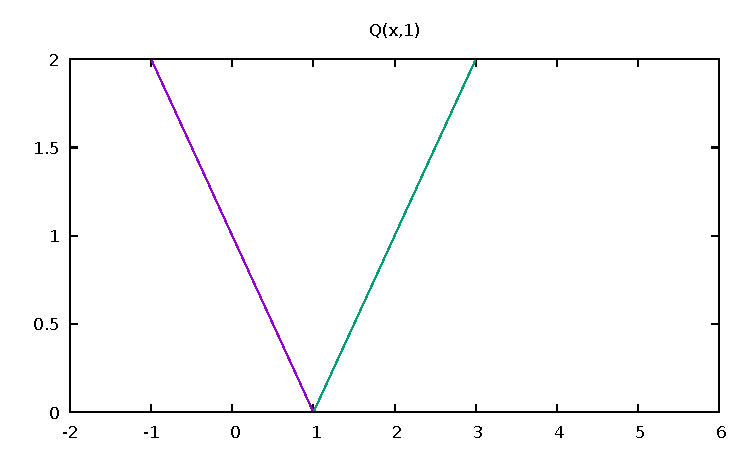
\includegraphics[width=\textwidth]{recourse_1.pdf}
\end{minipage}
\end{center}

\end{frame}

\begin{frame}
\frametitle{Graphically (cont'd)}

\begin{center}
\begin{minipage}{0.9\textwidth}
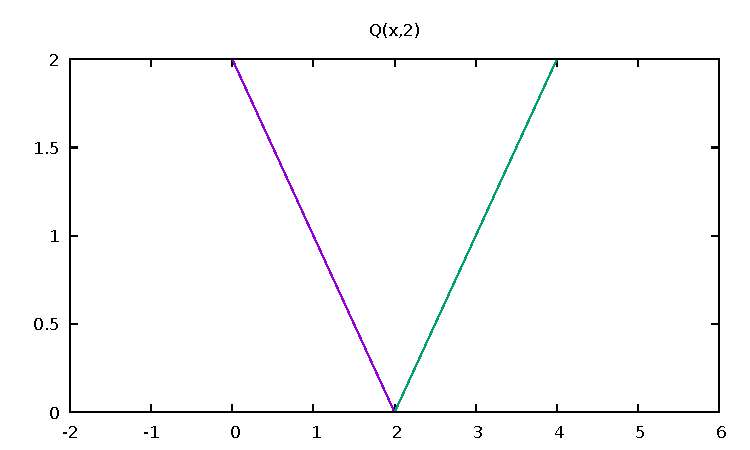
\includegraphics[width=\textwidth]{recourse_2.pdf}
\end{minipage}
\end{center}

\end{frame}

\begin{frame}
\frametitle{Graphically (cont'd)}

\begin{center}
\begin{minipage}{0.9\textwidth}
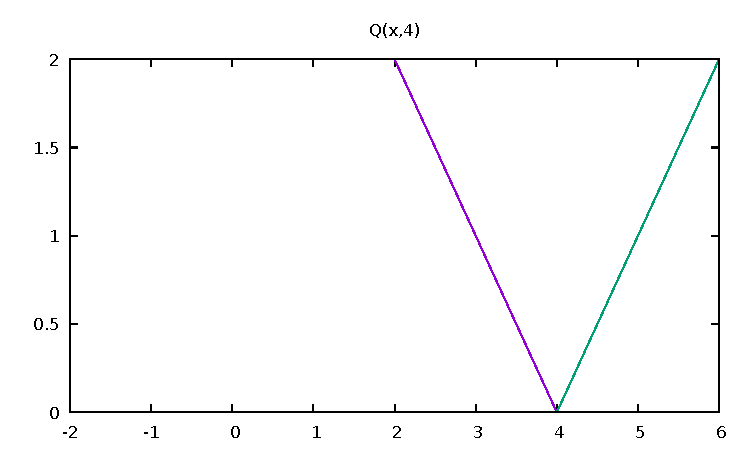
\includegraphics[width=\textwidth]{recourse_4.pdf}
\end{minipage}
\end{center}

\end{frame}

\begin{frame}
\frametitle{$\mathcal{Q}(x)$}

What about $\mathcal{Q}(x)$?

\mbox{}

Assume that the three realizations have the same probability.

\mbox{}

We have to consider 4 cases:
\begin{enumerate}
\item
$x \leq 1$: $\mathcal{Q}(x) = 7/3 - x$;
\item
$1 \leq x \leq 2$: $\mathcal{Q}(x) = 5/3-x/3$;
\item
$2 \leq x \leq 4$: $\mathcal{Q}(x) = x/3+1/3$;
\item
$4 \leq x$: $\mathcal{Q}(x) = x-7/3$;
\end{enumerate}

\end{frame}

\begin{frame}
\frametitle{Graphically}

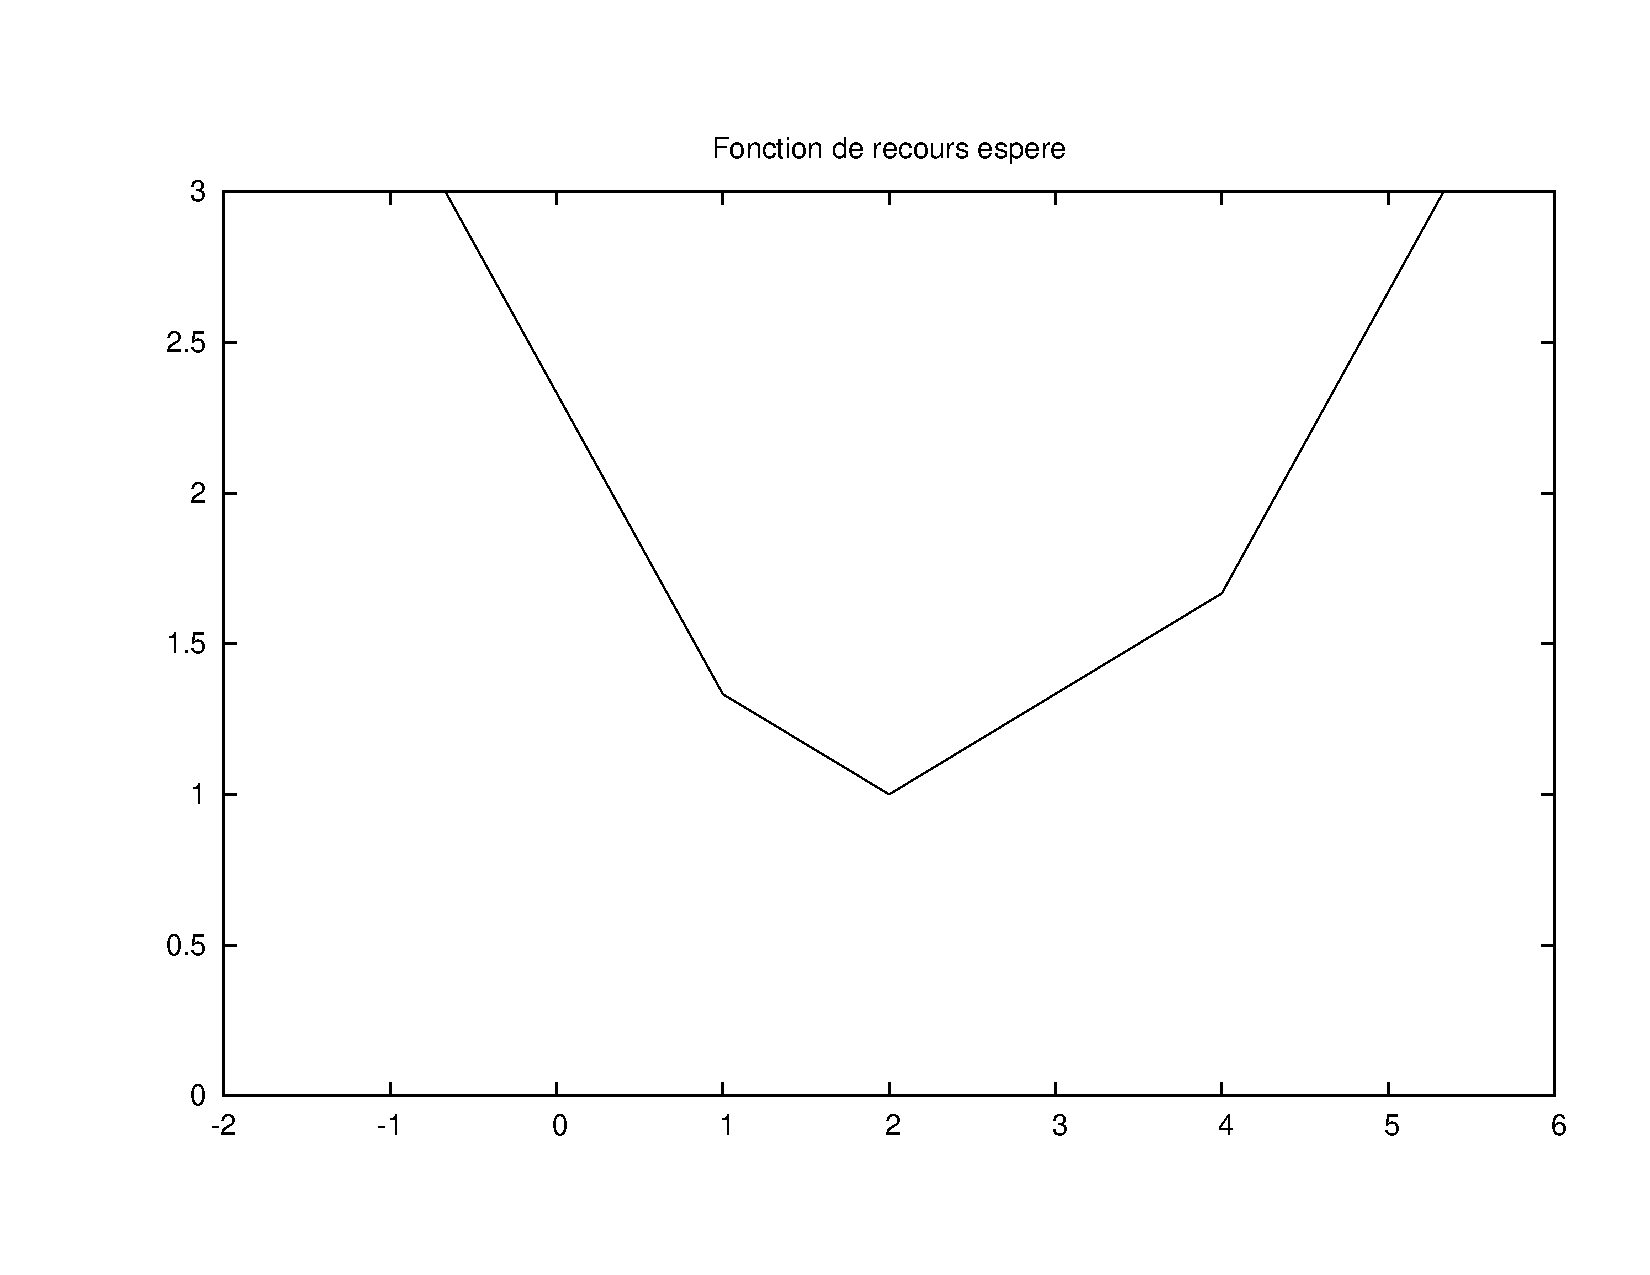
\includegraphics[width=0.9\textwidth]{recourse_all.pdf}

\end{frame}

\begin{frame}
\frametitle{Properties of $\mathcal{Q}(x)$}

We note that $\mathcal{Q}(x)$ is convex and piecewise linear.
As $\mathcal{Q}(x)$ is a finite weighted sum of piecewise linear functions when the support of $\bxi$ is finite, we have the following result.

\begin{theo}
For a stochastic program with fixed recourses where $\bxi$ has finite second-order moments,
\begin{enumerate}[(a)]
\item
$\mathcal{Q}(x)$ is a convex Lipschitz function and is finite over $K_2$;
\item
when $\bxi$ has a finite support, $\mathcal{Q}(x)$ is piecewise linear.
\end{enumerate}
\end{theo}

Reminder: a function $f$ is Lipschitz if there exists some $M < \infty$ such that for all $x$, $y$,
\[
|f(x)-f(y)| \leq M \| x-y \|.
\]

\end{frame}

\begin{frame}
\frametitle{Differentiability of the recourse}

Is $\mathcal{Q}(x)$ also differentiable?

\mbox{}

The recourse function is partially differentiable with respect to $x_j$ at $(\hat{x}, \hat{\xi})$ if the directional derivative exists for the direction $e_j$.
In other terms, there exists a function $\frac{\partial Q(x,\xi)}{\partial x_j}$ such that
\[
\frac{Q(\hat{x}+he_j,\hat{\xi}) - Q(\hat{x},\hat{\xi})}{h} =
\frac{\partial Q(x,\xi)}{\partial x_j} + \frac{\rho_j (\hat{x},
  \hat{\xi}; h)}{h},
\]
with
\[
\frac{\rho_j (\hat{x}, \hat{\xi}; h)}{h} \rightarrow 0, \mbox{ as } h\rightarrow 0.
\]

\mbox{}

We will assume from now that $\nabla_x Q(x, \xi) = \left( \frac{\partial
  Q(x,\xi)}{\partial x_1},\ldots, \frac{\partial
  Q(x,\xi)}{\partial x_n} \right)$ exists.

\end{frame}

\begin{frame}
\frametitle{Differentiability of the recourse (cont'd)}

What about the differentiability of $\mathcal{Q}(x)$?

\begin{align*}
\frac{\mathcal{Q}(\hat{x}+he_j) -
  \mathcal{Q}(\hat{x})}{h} &=
\int_{\Xi}
\frac{Q(\hat{x}+he_j,\xi) - Q(\hat{x},\xi)}{h} dP \\
&= \int_{\Xi \backslash N_{\delta}} \frac{\partial
  Q(\hat{x},\xi)}{\partial x_j} dP+ \int_{\Xi \backslash N_{\delta}}
\frac{\rho_j (\hat{x}, \xi; h)}{h} dP,
\end{align*}
where $N_{\delta}$ is measurable and $P[N_{\delta}] = 0$.
Therefore, we have
\begin{theo}
If $Q(x,\xi)$ if partially differentiable almost everywhere, if its partial derivative 
$\frac{\partial Q(\hat{x},\xi)}{\partial x_j}$ is integrable and if the residual satisfies
$(1/h) \int_{\Xi \backslash N_{\delta}} \rho_j (\hat{x}, \xi; h) dP \overset{h \rightarrow 0}{\rightarrow } 0$, then $\frac{\partial \mathcal{Q}(\hat{x})}{\partial x_j}$ exists and
\[
 \frac{\partial \mathcal{Q}(\hat{x})}{\partial x_j} =
 \int_{\Xi} \frac{\partial Q(\hat{x},\xi)}{\partial x_j} dP.
\]
\end{theo}

\end{frame}

\begin{frame}
\frametitle{Differentiability of the recourse: discrete case}

But how to prove $(1/p) \int_{\Xi
  \backslash N_{\delta}} \rho_j (\hat{x}, \xi; h) dP \overset{h
  \rightarrow 0}{\rightarrow } 0$?

\mbox{}

If we stay in the linear framework with fixed recourse, and vectors $\bxi$ with finite second-order moments, we have seen that for $\bxi$ with finite support, $\mathcal{Q}(x)$ is piecewise linear.
Therefore $\mathcal{Q}(x)$ is not differentiable.

\end{frame}

\begin{frame}
\frametitle{Differentiability of the recourse: continuous case}

If $\bxi$ is continuous, $\mathcal{Q}(x)$ is obtained as an integral over the $Q(x,\xi)$'s, that are not differentiable as they are piecewise linear given $\xi$.
However, it is $x$ that has to be fixed, not $\xi$.
It is possible to show that (the proof is quite technical)

\mbox{}

\begin{theo}
For a stochastic program with fixed recourse where $\bxi$ has finite second-order moments, if $\bxi$ is continuous, $\mathcal{Q}(x)$ is differentiable over $K_2$.
\end{theo}

\mbox{}

Intuitively, the function $\mathcal{Q}(x)$ is ``smoothed'' by the superposition of an infinite number of functions $Q(x,\xi)$.

\end{frame}

\begin{frame}
\frametitle{Two-stage non-linear problems}

Now consider the general program
\[
\min_{x \in X} E_{\bxi} [ f_0(x, \bxi) ] = \min_{x \in X}
E_{\bxi} [g_0(x,\bxi) + Q(x, \bxi)].
\]

\begin{theo}
If $g_0(\cdot,\xi)$ and $ Q(\cdot, \xi)$ are convex with respect to $x$, $\forall\ \xi \in \Xi$, and if $X$ is a convex set, the aforementioned program is convex.
\end{theo}
\begin{proof}
For $x$, $y \in X$, $\lambda \in (0,1)$ and $z = \lambda x +
(1-\lambda) y$, we have
\begin{multline*}
g_0(z, \xi) + Q(z, \xi) \\
\leq \lambda (g_0(x, \xi) + Q(x,
\xi)) + (1-\lambda)(g_0(y, \xi) + Q(y, \xi)).
\end{multline*}
The result follows by taking the expectation.
\end{proof}

\end{frame}

\begin{frame}
\frametitle{In a more standard form}

Inspired from Birge et Louveaux, Section~3.4.

\mbox{}

We consider the problem
\begin{align*}
\inf z &= f^1(x) + \mathcal{Q}(x), \\
\mbox{s.t. } & g_i^1(x) \leq 0,\ i = 1,\ldots,\overline{m}_1, \\
& g_i^1(x) = 0,\ i = \overline{m}_1+1,\ldots,m_1,
\end{align*}
where $\mathcal{Q}(x) = E_{\omega}[Q(x,\omega)]$ and
\begin{align*}
Q(x,\omega) &= \inf f^2(y(\omega), \omega), \\
\mbox{s.t. } & t_i^2(x, \omega) + g_i^2(y(\omega), \omega) \leq 0,\ i
= 1,\ldots,\overline{m}_2,\\
& t_i^2(x, \omega) + g_i^2(y(\omega), \omega) = 0,\ i =
\overline{m}_2+1,\ldots,m_2,
\end{align*}

\mbox{}

We say that the recourse is additive (why?).

\end{frame}

\begin{frame}
\frametitle{In a more standard form (cont'd)}

The functions $f^2(\cdot, \omega)$, $t_i^2(\cdot, \omega)$, and $g_i^2(\cdot, \omega)$ are continuous for any given $\omega$, and measurable w.r.t. $\omega$ for any given first argument.
This allows to prove that $Q(x,\omega)$ is measurable, and therefore that $\mathcal{Q}(x)$ is well defined.

\mbox{}

Reintroduce $K_1$, $K_2(\omega)$ and $K_2$.

\begin{align*}
K_1 & = \lbrace x \ |\ g_i^1(x) \leq 0,\ i =
1,\ldots,\overline{m}_1, \\
& \quad \qquad g_i^1(x) = 0,\ i = \overline{m}_1+1,\ldots,m_1 \rbrace, \\
K_2(\omega) & = \lbrace x \ |\ \exists\, y(\omega) \mbox{ t.q. }
 t_i^2(x, \omega) + g_i^2(y(\omega), \omega) \leq 0,\ i
= 1,\ldots,\overline{m}_2,\\
& \quad \qquad t_i^2(x, \omega) + g_i^2(y(\omega), \omega) = 0, \ i =
\overline{m}_2+1,\ldots,m_2 \rbrace, \\
K_2 & = \lbrace x \ |\ \mathcal{Q}(x) < \infty \rbrace.
\end{align*}

\end{frame}

\begin{frame}
\frametitle{Remarks}

The formulation is not yet totally general.
We will consider more general forms when we will discuss sampling techniques.

\mbox{}

Here, there is no more fixed recourse, but the first-stage decision $x$ acts separately in the constraints.
Goal: extend the previous results.

\mbox{}

Questions: convexity, differentiability, optimality.
We should also consider the concept of lower semi-continuity.

\end{frame}

\end{document}